\documentclass[a11paper, 11pt]{article}

\usepackage{libs/document}
\usepackage{libs/titlepage}
\usepackage{listings}
\usepackage{graphicx}
\usepackage{array}
% \usepackage{minted}
\usepackage{multicol}
\usepackage[T1]{fontenc}
\usepackage[french]{babel}

\addbibresource{refs/bibliography.bib}
% \nofiles


\lstset{%
        inputencoding=utf8,
        extendedchars=true,
        basicstyle=\footnotesize\ttfamily,
        showstringspaces=false,
        showspaces=false,
        % numbers=left,
        % numberstyle=\footnotesize,
        numbersep=9pt,
        tabsize=2,
        breaklines=true,
        showtabs=false,
        captionpos=b,
        literate=%
        {é}{{\'{e}}}1
        {è}{{\`{e}}}1
        {ê}{{\^{e}}}1
        {ë}{{\¨{e}}}1
        {É}{{\'{E}}}1
        {Ê}{{\^{E}}}1
        {û}{{\^{u}}}1
        {ù}{{\`{u}}}1
        {ú}{{\'{u}}}1
        {â}{{\^{a}}}1
        {à}{{\`{a}}}1
        {À}{{\`{A}}}1
        {á}{{\'{a}}}1
        {ã}{{\~{a}}}1
        {Á}{{\'{A}}}1
        {Â}{{\^{A}}}1
        {Ã}{{\~{A}}}1
        {ç}{{\c{c}}}1
        {Ç}{{\c{C}}}1
        {õ}{{\~{o}}}1
        {ó}{{\'{o}}}1
        {ô}{{\^{o}}}1
        {Õ}{{\~{O}}}1
        {Ó}{{\'{O}}}1
        {Ô}{{\^{O}}}1
        {î}{{\^{i}}}1
        {Î}{{\^{I}}}1
        {í}{{\'{i}}}1
        {Í}{{\~{Í}}}1
}
\renewcommand\lstlistingname{Algorithme}

% \institution{Université de Sherbrooke}
% \faculty{Faculté de génie}
% \department{Département de génie électrique et de génie informatique}
\title{Rapport d'APP}
\classnb{APP2}
\class{Programmation et algorithmes}
\author{
  \addtolength{\tabcolsep}{-0.4em}
  \begin{tabular}{rcl} % Ajouter des auteurs au besoin
  Benjamin Chaussé     & -- & chab1704 \\
  Guillaume Malgorn    & -- & malg1503 \\
  \end{tabular}
}
\teacher{Charles-Antoine Brunet} % TODO: Est-ce le bon prof pour le rapport?
% \location{Sherbrooke}
% \date{\today}

\begin{document}
\maketitle
\tableofcontents
\newpage

\section{Introduction}

XY-calculus est une entreprise spécialisée dans des calculs mathématiques
allant de simple à complexe. En effet, les mathématiques est une science
présente dans les civilisations depuis des millénaires. Elles sont la
base de la compréhension du monde. Elles sont utilisées dans chaque
aspect de la vie. Elles sont également étroitement reliées à
l’informatique. XY-calculus utilise les mathématiques et les
l’informatique afin de créer une librairie de fonctions mathématiques
pour rendre plus simple les calculs liés à ces fonctions. Notre mandat
est de faire le programme en langage C de 6 fonctions mathématiques:
recherche d’un caractère, détection de palindrome, calcul du sinus et du
cosinus, addition de matrice et multiplication de matrices carrées. Nous
avons également le mandat de faire leurs pseudocodes ou leurs diagrammes
d’activité ainsi que leurs plans de tests.

\section{Opérations sur du texte}
\subsection{Trouver un caractère}

\begin{multicols}{2}

\begin{lstlisting}[caption=Pseudocode de la fonction findChar]
FONCTION findChar(mot[],target) : i
  // mot[] (liste de caractères): mot à analyser
  // target (caractère): lettre que l'on souhaite identifier
  // i (entier): position de la lettre que l'on souhaite trouver
DÉBUT
    // len (entier) : longueur du mot choisi
    len := 0
    TANT QUE (mot[i] != '\0')
        len = len + 1
    POUR i:=0 À i >= len PAR PAS DE 1
        SI (mot[i] == target) ALORS
            Écrire i à l'écran
    SINON
        Écrire -1 à l'écran
FIN
\end{lstlisting}

% TODO: mettre les all CAPS en gras
% TODO: vérifier la syntaxe de écrire à l'écran

\columnbreak

\begin{lstlisting}[language=C,caption=Fonction findChar écrite en C]
int findChar(char *mot,char target){
  int len = 0;
  while (mot[len]!= '\0'){
    len ++;
  }
  for (int i=0;i<len;i++){
    if (mot[i] == target){
      return i;
    }
  }
  return -1;
}
\end{lstlisting}

\end{multicols}

Afin de s'assurer du bon fonctionnement du programme, nous pouvons vérifier
qu'il retourne une série de valeurs connues et attendues dans différents
scénarios et cas limites. Parmi ceux-ci, les tests vérifieront comment la
fonction gère l'inexistance du caractère dans un mot, l'existance d'un
caractère à la fin du mot, l'existance du caractère à la première position
puis l'utilisation du plus long mot qui existe.

\begin{table}[H]
  \centering
  \caption{Plan de test de la fonction findChar}
  \label{tab:findChar-tests}
  \begin{tabular}{lll}
  \toprule
  Mot donné                & Caractère recherché & Résultat attendu \\
  \midrule
  anticonstitutionellement & n                   & 1                \\
  bonjour                  & e                   & -1               \\
  bonjour                  & r                   & 6                \\
  allocommentcava          & a                   & 0                \\
  \bottomrule
  \end{tabular}
\end{table}


\subsection{Reconnaissance de palindromes}

\begin{multicols}{2}

\begin{figure}[H]
  \centering
  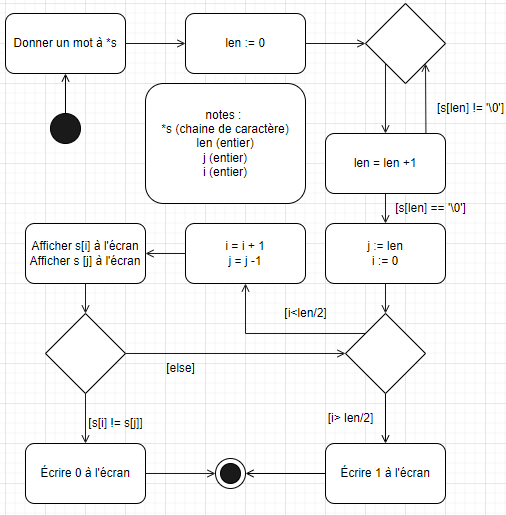
\includegraphics[width=\linewidth]{figures/palindrome-uml.png}
  \caption{Diagrame d'activité de la fonction palindrome}
  \label{fig:pal-uml}
\end{figure}

\columnbreak

\begin{lstlisting}[caption=Fonction palindrome écrite en C]
int palindrome(char *s){
  int len = 0;
  while (s[len]!= '\0'){
    len ++;
  }
  int j = len;
  for (int i=0; i<len/2;i++){
    j--;
    printf("\%c-",s[i]);
    printf("\%c\n",s[j]);
    if (s[i] != s[j]){
      return 0;
    }
  }
  return 1;
}
\end{lstlisting}

\end{multicols}

Afin d'établir le bon fonctionnement de la fonction palindrome, la fonction
sera testée contre des mots ayant un nombre de caractère impaire qui sont des
palindromes, des mots ayant un nombre pair de caractères qui sont des
palindromes et des mots qui ne sont tout simplement pas des palindromes.

\begin{table}[H]
  \centering
  \caption{Plan de test des fonctions trigonométriques}
  \label{tab:pal-tests}
  \begin{tabular}{ll}
    \toprule
    Mot choisi & Résultat attendu \\
    \midrule
    tenet & 1 \\
    automobile & 0 \\
    redder & 1 \\
    \bottomrule
  \end{tabular}
\end{table}


\section{Opérations trigonométriques}

Les fonctions trigonométriques sinus et cosinus sont calculées en faisant appel
au séries de Taylor. Dans les deux cas, les sommations font appel à des
exposants pour leurs calculs. Afin d'éviter la redondance, une fonction
\verb|pow| a été écrite afin d'être utilisée dans les deux cas. Aussi, dans le
but de minimiser le nombre d'opérations que l'ordinateur accompli, cette
fonction emploi l'algorithme de l'exponentiation par carrés\cite{square-exp}.
La voici ainsi que le pseudocode décrivant sont fonctionnement.
% TODO: Write reference

\begin{multicols}{2}
\begin{lstlisting}[caption=Pseudocode de la fonction pow]
FONCTION pow(b,e)
  // b: base de l'exposant
  // e: puissance de l'exposant
DEBUT
  SI e=1 ALORS
    Écrire à l'écran b
  SI e%2=0 ALORS
    pow(b*b, e/2)
  SI e%2=1 ALORS
    pow(b*b, e/2)
FIN
\end{lstlisting}
\columnbreak
\begin{lstlisting}[caption=Fonction pow écrite en C]
 double pow(double b, int e){
  if (e==1){
    return b;
  } else if (e%2==0){
    return pow(b*b,e/2);
  } else {
    return b * pow(b*b, e/2);
  }
}
\end{lstlisting}
\end{multicols}

Aussi, vu la proximité de la relation entre la foncion cosinus et sinus, nous
pouvons concevoir un plan de test qui sera utile au deux fonctions afin de
vérifier leur bon fonctionnement.

\begin{table}[H]
  \centering
  \caption{Plan de test des fonctions trigonométriques}
  \label{tab:trig-tests}
  \begin{tabular}{lll}
    \toprule
    Valeur donnée  & Sinus attendu & Cosinus attendu \\
    \midrule
    $1$            & \num{0.8415}  & \num{0.5403}    \\
    $0$            & \num{0}       & \num{1}         \\
    $\pi/4$        & \num{0.7071}  & \num{0.7071}    \\
    $\pi/2$        & \num{1}       & \num{0}         \\
    \bottomrule
  \end{tabular}

\end{table}

\newpage
\subsection{Sinus}

\begin{multicols}{2}

\begin{lstlisting}[caption=Pseudocode de la fonction sinus]
FONCTION sin(input, precision) : ttl
	// input : valeur du sinus
	// precision (entier) : precision du sinus
	// ttl (réel) : valeur que le sinus nous retourne
DEBUT
  // denom (entier) := 1
  // ttl (réel) := input
  // num (réel) : valeur du numérateur
  // i (entier)
  // pow : fonction de la puissance
  // pow : fonction de la puissance
POUR i = 3 À i<(2*precision)+2 PAR PAS DE 2
  num := pow(input,i)
  denom = denom * (i*(i-1))
  SI (i-1)/2 %2 == 1 ALORS
    ttl = ttl - (num/denom)
  ELSE
    ttl = ttl + (num/denom)
  Écrire ttl à l'écran
FIN
\end{lstlisting}

\columnbreak

\begin{lstlisting}[caption=Fonction sinus écrite en C]
double sin(double input, int precision){
  double ttl = input;
  int denom = 1;
  double num;
  for (int i=3;i<(2*precision)+2;i+=2) {
    num = pow(input,i);
    denom *= i*(i-1);
    ttl += ((i-1)/2 %2 == 1) ? -num/denom : num/denom;
  }
  return ttl;
}
\end{lstlisting}

\end{multicols}

\newpage
\subsection{Cosinus}

\begin{multicols}{2}

\begin{figure}[H]
  \centering
  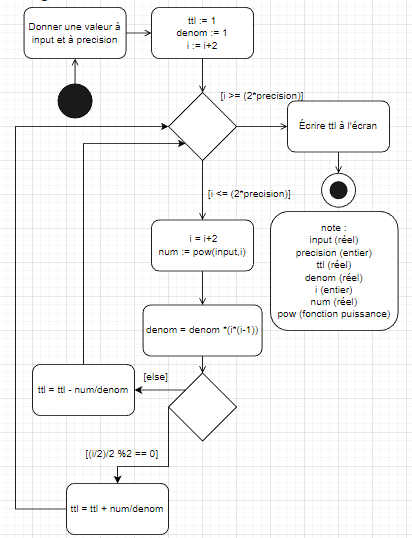
\includegraphics[width=\linewidth]{figures/cosinus-uml.png}
  \caption{Diagramme d'activité de la fonction Cosinus}
  \label{fig:cos-uml}
\end{figure}

\columnbreak

\begin{lstlisting}[caption=Fonction cosinus écrite en C]
double cos(double input, int precision){
  double ttl = 1;
  int denom = 1;
  double num;
  for (int i=2;i<=(2*precision);i+=2){
    num = pow(input,i);
    denom *= i*(i-1);
    ttl += ( (i/2)%2 == 0 ) ? num/denom : -num/denom;
  }
  return ttl;
}
\end{lstlisting}

\end{multicols}

\newpage
\section{Opérations matricielles}
\subsection{Addition de matrices}

\begin{multicols}{2}
  \begin{figure}[H]
  \centering
  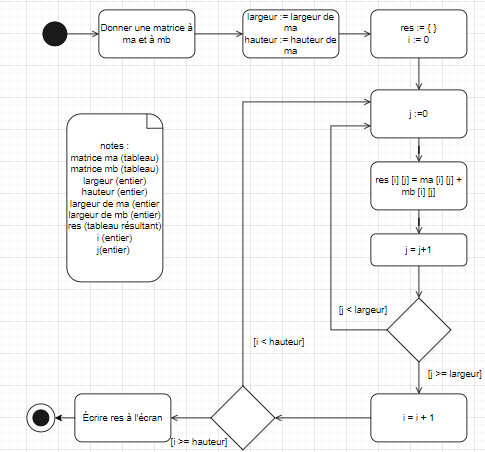
\includegraphics[width=\linewidth]{figures/matAdd-uml.png}
  \caption{Diagramme d'activité de la fonction matAdd}
  \label{fig:matAdd-uml}
\end{figure}

\columnbreak

\begin{lstlisting}[caption=Fonction matAdd écrite en C]
int *matAdd(int *ma, int *mb, int w, int h){
  int res[h][w];
  for (int i=0;i<w;i++){
    for (int j=0;j<h;j++){
      res[i][j] = *(ma+(i*h)+j) + *(mb+(i*h)+j);
    }
  }
    return *res;
}
\end{lstlisting}
\end{multicols}

Afin de vérifier le bon fonctionnement de la fonction matAdd, une somme de 2
matrices 3x2 sera effectuée.

\begin{table}[H]
  \centering
  \caption{Plan de test de la fonction matAdd}
  \label{tab-tests}
  \begin{tabular}{p{2.5cm}p{2.5cm}p{3cm}}
    \toprule
    Matrice A & Matrice B & Résultat attendu \\
    \midrule
    \[
    \left[ {\begin{array}{cc}
    {1} & {2} \\
    {3} & {4} \\
    {5} & {6} \\
            \end{array} } \right]
    \] & \[
    \left[ {\begin{array}{cc}
    {6} & {5} \\
    {4} & {3} \\
    {2} & {1} \\
            \end{array} } \right]
    \] & \[
    \left[ {\begin{array}{cc}
    {7} & {7} \\
    {7} & {7} \\
    {7} & {7} \\
            \end{array} } \right]
    \] \\
    \bottomrule
  \end{tabular}
\end{table}


\newpage
\subsection{Multiplication de matrices}

\begin{multicols}{2}
\begin{lstlisting}[caption=Pseudocode de la fonction matMult]
FONCTION matMult(ma[][], mb[][], h1, c, w2): m[][]
  // ma[] : Première matrice de l'opération (matrice A)
  // mb[] : Deuxième matrice de l'opération (matrice B)
  // ha   : Hauteur (nombre de rangées) de la matrice A
  // wb   : Largeur (nombre de colonnes) de la matrice B
  // c    : Dimension commune des deux matrices (largeur A et hauteur B)
DEBUT
  // Matrice vierge dans laquelle le produit sera calculé:
  res[ha][wb] := {}
  POUR i:= 0 À i<ha
    POUR j:=0 À j<wb
      cell := 0
      POUR k:=0 À k<c
        // On ajoute le produit des paires de chiffre au total de la cellule
        cell := cell + ( ma[i][k] * mb[k][j] )
      res[i][j] = cell
  Écrire res à l'écran
FIN
\end{lstlisting}
\columnbreak
\begin{lstlisting}[caption=Fonction matMult écrite en C]
int *matMult(int *ma, int *mb, int ha, int c, int wb){
  int res[ha][wb];
  for (int i=0;i<ha;i++){
    for (int j=0;j<wb;j++){
      int cell = 0;
      for (int k=0;k<c;k++){
        cell += *((ma+i*c)+k) * *((mb+wb*k)+j);
      }
      res[i][j] = cell;
    }
  }
  return *res;
}
\end{lstlisting}

\end{multicols}

\newpage
Afin de vérifier le bon fonctionnement de la fonction, deux matrices de
dimensions 3 seront multipliées ensemble.

\begin{table}[H]
  \centering
  \caption{Plan de test de la fonction matAdd}
  \label{tab-tests}
  \begin{tabular}{p{2.5cm}p{2.5cm}p{3cm}}
    \toprule
    Matrice A & Matrice B & Résultat attendu \\
    \midrule
    \[
    \left[ {\begin{array}{ccc}
    {1} & {2} & {3}\\
    {4} & {5} & {6}\\
    {7} & {8} & {9}\\
            \end{array} } \right]
    \] & \[
    \left[ {\begin{array}{ccc}
    {2} & {0} & {0}\\
    {0} & {2} & {0}\\
    {0} & {0} & {2}\\
            \end{array} } \right]
    \] & \[
    \left[ {\begin{array}{ccc}
    {2} & {4} & {6}\\
    {8} & {10} & {12}\\
    {14} & {16} & {19}\\
            \end{array} } \right]
    \] \\
    \bottomrule
  \end{tabular}
\end{table}



\section{Conclusion}

Enfin, nous avons pu voir les différentes programmations en C des
fonctions demandées ainsi que leurs plans de tests et leurs
pseudocode/diagramme d’activité associé. Nous avons rencontré quelques
difficultés notamment sur les programmes liés aux matrices ainsi que sur le
formalisme des pseudocodes et des diagrammes d’activité. Nous avons dû nous
reprendre plusieurs fois pour avoir des pseudocodes et des diagrammes
d’activité respectant les critères exigés.

\newpage
\printbibliography[heading=bibintoc]
\end{document}
